\documentclass[10pt, aspectratio=169]{beamer}

% --- Theme ---
\usetheme{metropolis} 
\usecolortheme{dolphin}

% --- Comentaris a color ---
\usepackage{xcolor}
\newcommand{\pau}[1]{{\color{red}{#1}}}


% --- Packages ---
\usepackage{tikz}
\usepackage{booktabs} % For nice tables
\usepackage{graphicx}
\usepackage{amsmath}  % For math formatting
\usepackage{hyperref}
\hypersetup{colorlinks=true, linkcolor=blue, urlcolor=blue}

% --- Metadata ---
\title[ICE Champions League]{ICE Champions League}
\subtitle{An End-to-End Pipeline for Foosball Positional Analytics}
\author{Pau Grèbol Tomàs}
\institute[ICE-CSIC/IEEC]{\href{mailto:grebol@ice.csic.es}{grebol@ice.csic.es} \\ ICE-CSIC/IEEC}
\date{\today}

\begin{document}

% --- Title Slide ---
\begin{frame}
    \titlepage
\end{frame}

% --- Table of Contents ---
\begin{frame}{Outline}
    \tableofcontents
\end{frame}

% ============================================================================
% SECTION 1: GOAL
% ============================================================================
\section{Introduction and goal}

\begin{frame}{The ICE Champions League}
\fontsize{7pt}{9pt}\selectfont


    \textbf{Context \& The "Experimental Setup"}
    \begin{itemize}
        \item \textbf{The Environment:} Daily 2v2 foosball matches among PhD students at ICE-CSIC.
        \item \textbf{The Dataset:} A rich historical record of $>1000$ matches.
        \item \textbf{The Challenge:} How do we objectively quantify individual player skill in a team-based, dynamic game?
    \end{itemize}

    \vspace{0.8em}

    \textbf{The Solution: A Custom Python Pipeline}
    \begin{itemize}
        \item Automatically compiles and processes seasonal match results. Prepared to be run from terminal with a simple command.
        \item Adapts the \textbf{ELO rating system} to estimate individual player potential.
        \item Computes player synergies to visualize team performance.
        \item Creates plots to visualize individual and team performance.
        \item Ultimately, feeds match data to a winning-predicting machine learning model.
    \end{itemize}

    \vspace{0.8em}

    % Using a block naturally draws the eye to the goals of your talk
    \begin{block}{Objectives of this Presentation}
        \begin{enumerate}
            \item Explain the mathematical framework of our ELO computation.
            \item Analyze statistical trends and insights from the $>1000$ match dataset.
            \item \textit{Note:} The entire Python pipeline is open-source and available on its \href{https://www.github.com/pgrebolt/ICEChampionsLeague}{GitHub repository}.
        \end{enumerate}
    \end{block}

\end{frame}

% Slide 2: The Dataset & Observables (Briefly showing what data is recorded: Player A, Player B vs Player C, Player D, Score, Date).
\begin{frame}{The game and the dataset}

	\begin{columns}
        \column{0.5\textwidth}
        \begin{center}
        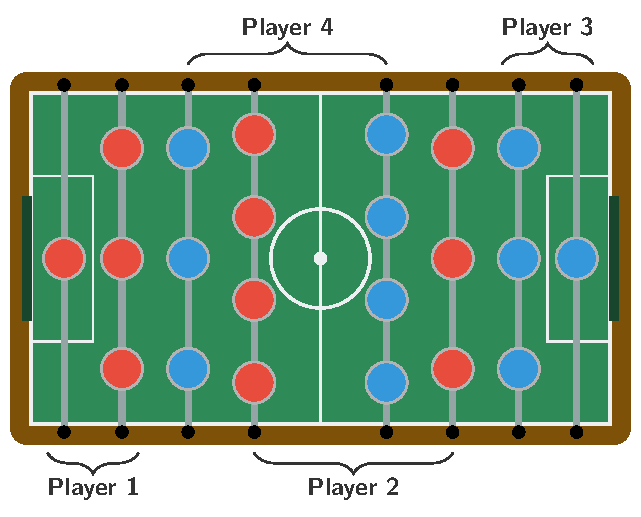
\includegraphics[width=0.55\textwidth]{table_scheme.pdf}
        \end{center}
        \footnotesize{
        \textbf{Rules}
        \begin{itemize}
            \item 2 teams, 2 players per team
            \item Line-up cannot be changed once the game has started
            \item First team to score 3 goals wins. No time limit
            \item Own goals are valid
            \item Players can interchange teams at the start of a new game
        \end{itemize}
}
		\column{0.5\textwidth}
        
        \footnotesize{
        \textbf{Dataset}
        \begin{itemize}
            \item Columns: name of players, goals scored per player, final result (to account for own goals)
            \item 29 individual players
            \item Results recorded per season (1 season $\simeq$ 3 months $\simeq$ 60 games)
            \item The total amount of recorded games across all seasons is $>1000$
            \item Data stored in a shared Google Sheets, so that results can be recorded at the end of each game from a smartphone
        \end{itemize}
        }
        		\resizebox{\textwidth}{!}{%
        \begin{tabular}{ccccccccccc}
        \toprule
        \textbf{Dia} & \textbf{Jugador 1} & \textbf{Jugador 2} & \textbf{Jugador 3} & \textbf{Jugador 4} & \textbf{Gols 1} & \textbf{Gols 2} & \textbf{Gols 3} & \textbf{Gols 4} & \textbf{Local} & \textbf{Visitant} \\ \midrule
        1 & Luis & Dani & Antía & Guille & 1 & 2 &  & 1 & 3 & 1 \\ 
        1 & Dani & Rebeca & Antía & Pedro & 1 & 1 & 2 & 1 & 2 & 3 \\ 
        2 & Guille & Pau & Víctor & Luis &  & 3 & 2 &  & 3 & 2 \\ 
        2 & Guille & Pau & Pedro & Dani & 1 & 1 & 1 & 1 & 2 & 3 \\ 
        \vdots & \vdots & \vdots & \vdots & \vdots & \vdots & \vdots & \vdots & & \\ \bottomrule
        \end{tabular} 
        }
        
    \end{columns}
    
\end{frame}

% ============================================================================
% SECTION 2: THE MATHEMATICAL FRAMEWORK (ELO)
% Physicists will love this part. Treat ELO as a state-updating algorithm.
% ============================================================================
\section{Mathematical Framework: Adapting ELO for 2v2}

% --- FRAME 1 ---
\begin{frame}{The ELO Rating System}

\fontsize{7pt}{9pt}\selectfont

\begin{columns}
\begin{column}{0.6\textwidth}
    \textbf{Standard ELO Framework}
    \begin{itemize}
        \item Designed to rank players despite different number of games played.
        \item Upsets (low-tier beating high-tier) cause massive rating shifts, while expected outcomes cause minimal shifts.
    \end{itemize}
    
        \textbf{Positional ELO rating:} Every player ($p$) tracks \textbf{two independent ELO ratings}: Offense and Defense.
        %\item The "Opponent ELO" is computed as a weighted average of the opponent team, factoring in their historical matches in those specific positions.

    \textbf{Win Probability:} For Team A ($s_A$) and Team B ($s_B$), the expected win probability for A is modeled as a logistic function:
        $$P_A(s_A, s_B) = \frac{1}{1 + 10^{(s_B - s_A) / 400}}.$$
        
\end{column}
\begin{column}{0.4\textwidth}

\begin{center}
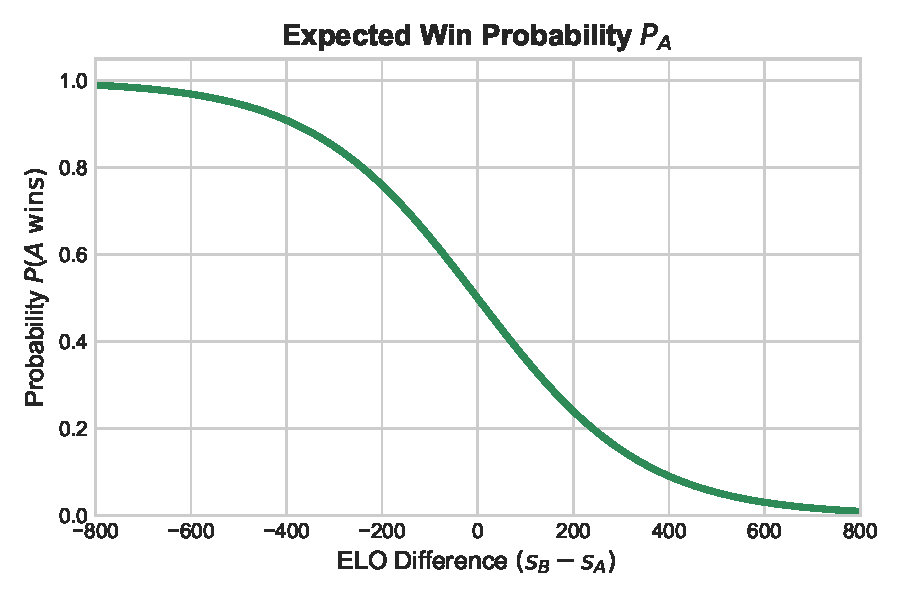
\includegraphics[width = 0.9\textwidth, keepaspectratio]{elo_logistic_curve.pdf}
\end{center}

\end{column}
\end{columns}


\begin{alertblock}{Team ELO}
        The team ELO is computed as a weighted mean of the players' individual ELOs based on their positional experience:
        $$ s_A = \frac{1}{G_A} \sum_{p \in A} G_{p, i}s_p , \quad G_A = G_{p, 1} + G_{p, 2}$$
        
        where $G_{p,i}$ is the number of games played by player $p$ in their current position $i$, $G_A$ is their total games played by both team players, and $s_p$ is their current ELO rating.
\end{alertblock}


\end{frame}

\begin{frame}{The ELO Rating System}

\begin{alertblock}{Updating the ELO}
        After a match, the ELO rating of a player ($s_p$) are updated based on the actual outcome vs. expected:
		$$\boxed{s_p \leftarrow s_p + K \cdot R_p \cdot (W - P_T)}$$
		where $K=30$ is the maximum rating change (arbitrary value), $R_p$ is a performance factor, $W=1$ ($W=0$) in a win (lose) scenario, and $P_T$ is the team probability of winning. For each position ($i$), starting ELO is $s_{p, i} = 1000$.
\end{alertblock}
\end{frame}

% --- FRAME 2 ---
\begin{frame}{The ELO Rating System}

%\fontsize{7pt}{9pt}\selectfont
    
    \begin{alertblock}{The Performance Weight ($R_p$)}
        In traditional ELO, teammates gain or lose the exact same number of points. In our case, a normalized weight, $R_{p, i}$, is introduced to account of a player $p$ individual performance in position $i$ during the game:
    
    $$ R_{p, i} = \frac{r_{p, i}}{\sum_{k \in \text{Team}} r_{k, j}} $$
    
    Here, $r_{p, i}$ is the raw performance score of player $p$ in position $i$. The denominator normalizes $R_{p, i}$ to the overall team performance ($\sum R = 1$).
    \end{alertblock}

\end{frame}



% --- FRAME 3 ---
\begin{frame}{Quantifying Individual Performance ($r_i$)}
    How do we measure if a player had a "good game" in a 3-goal match?
    
    \vspace{0.5em}
    \textbf{Attacker Performance:}
    $$ r_i (\text{Atk}) =  \mu \cdot \left(\frac{\text{Goals Scored}}{3} \right) + \lambda \cdot \left( 1- \frac{\text{Goals Received}}{3} \right) $$

    \vspace{0.5em}
    \textbf{Defender Performance:}
    $$ r_i (\text{Def}) = \mu \cdot \left( 1 - \frac{\text{Goals Received}}{3} \right) + \lambda \cdot \left( \frac{\text{Goals Scored}}{3} \right) $$

    \vspace{0.5em}
    \begin{itemize}
        \item $\mu = 0.7$: Weight of primary duty (Attacker scoring / Defender defending).
        \item $\lambda = 0.3$: Weight of secondary duty (Cross-contribution).
    \end{itemize}

\end{frame}

% --- FRAME 4 ---
\begin{frame}{Performance factors in defeat cases}

    Consider the definition of $R_p$:
    $$ R_{p, i} = \frac{r_{p, i}}{\sum_{k \in \text{Team}} r_{k, j}} $$
    
    Consider that a team loses, with defender conceding 3 goals and scoring 0. With that definition, and the definition of $r_i$ we would get  $r_i = 0 \implies R_i = 0$. The defender would not lose any ELO points despite a terrible performance.

	\textit{Solution:}
    To properly penalize poor performance in a \textbf{loss}, the metric is \textbf{inverted} in case of defeat:
    $$ r_i' = 1 - r_i \quad \implies \quad R'_{p,i} = \frac{r'_i}{\sum_k r'_k} $$
    
     \textbf{Regularization (Minimum Floor)}
    \begin{itemize}
        \item An absolute minimum boundary is imposed: $r_{p, i} \geq 0.1 \leftrightarrow r'_{p, i} \leq 0.9$.
        \item This mathematically prevents divisions by zero and ensures a minimal contribution by each player.
    \end{itemize}


\end{frame}

\begin{frame}{Weighted ELO}
    \begin{alertblock}{}
    A combined ELO to find the most complete player. It is a weighted sum of the games played in each position and the corresponding ELO in that position:
        $$ s_{p, w} = \left( \frac{G_{p, \text{Atk}}}{G_{p, \text{tot}}} \right) s_{p, \text{atk}} + \left( \frac{G_{p, \text{Def}}}{G_{p, \text{tot}}} \right) s_{p, \text{def}} $$
    
    \scriptsize{\textit{Note: Until the player has played at least one game in each position, its weighted ELO is set at $ \tilde{s}_{p, w} = 1000$.}}
    \end{alertblock}

\end{frame}

% --- FRAME 5 ---
\begin{frame}{Summary of ELO computation}
	\centering
	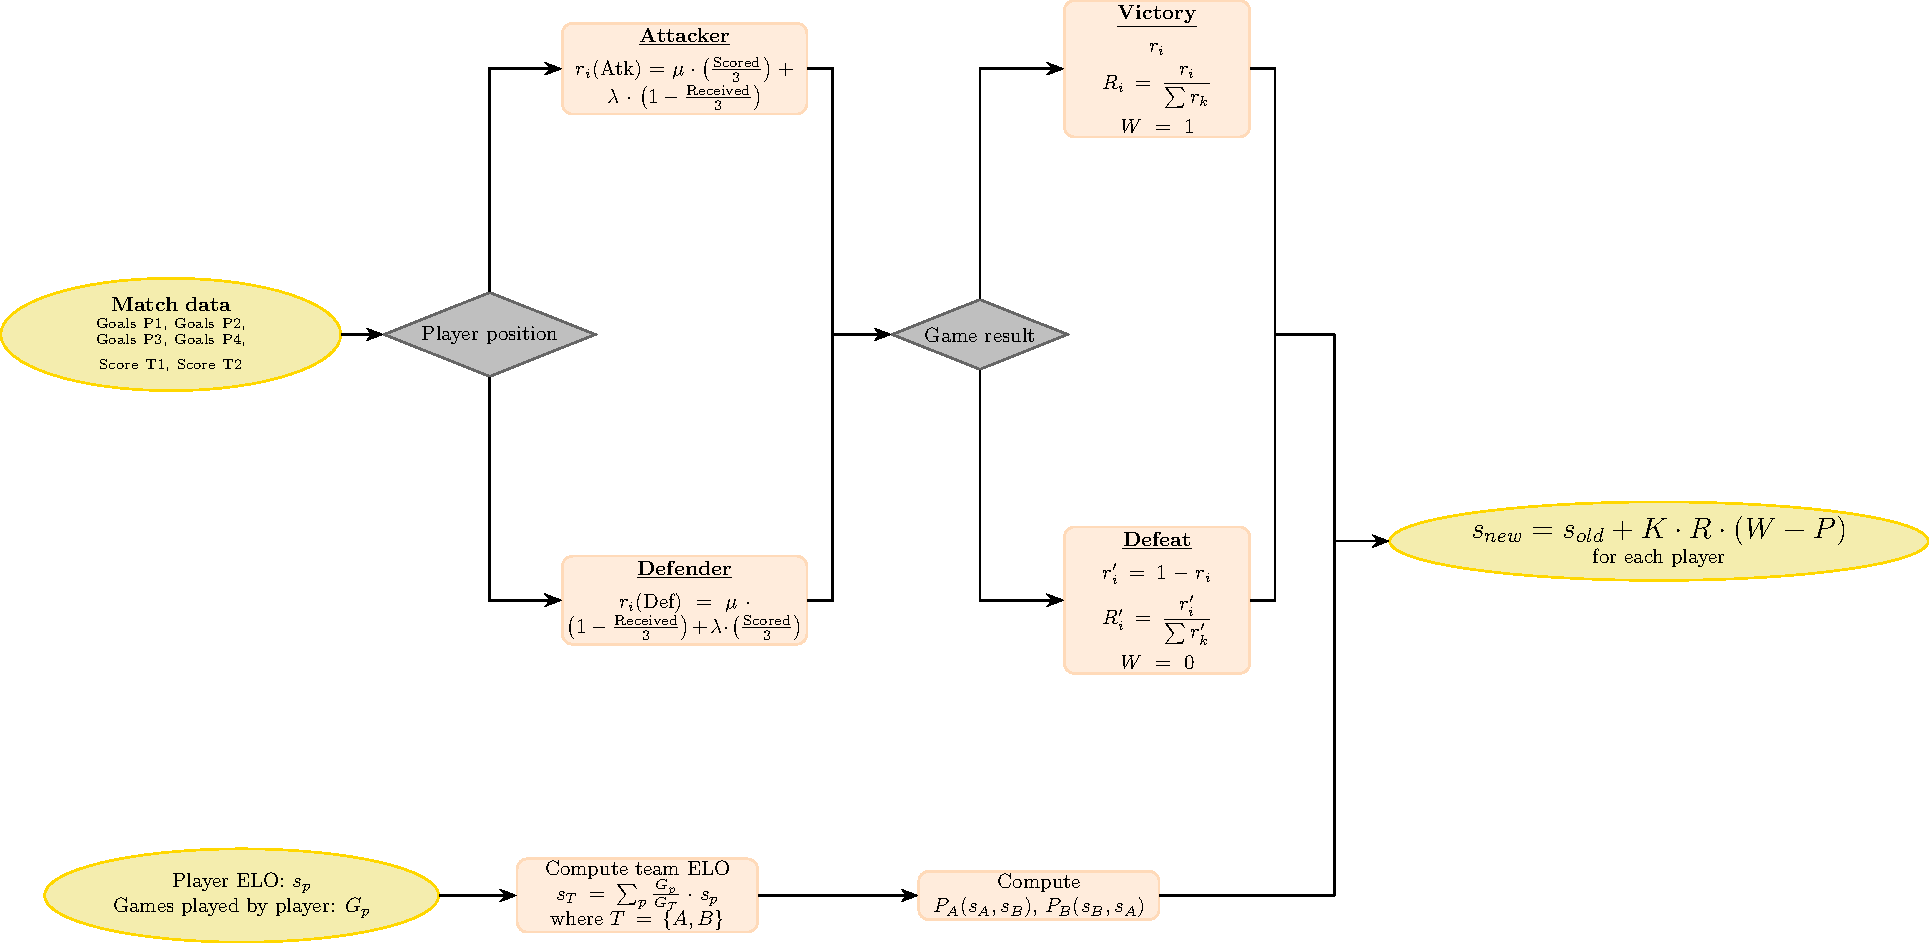
\includegraphics[width = 1.05\textwidth]{ELO_update_workflow.pdf}
\end{frame}

\begin{frame}{Hands-on practical example}
\fontsize{7pt}{9pt}\selectfont
\textbf{Initial State:} $K=30, \mu=0.7, \lambda=0.3$. \hfill \textbf{Score:} 3--1 (Team A Victory)
    
    \vspace{0.1em}
    % --- Step 1: Probability Calculation ---
    \begin{block}{Expected Probability ($P_A$)}
        Given $s_A = 1004$ and $s_B = 1268$, the system predicts a significant advantage for Team B:
        $$ P_A = \frac{1}{1 + 10^{(1268-1004)/400}} \approx \mathbf{0.18}$$
    \end{block}

	\vspace{-2em}
    \begin{columns}[T]
        % --- Winning Team A ---
        \begin{column}{0.4\textwidth}
            \begin{alertblock}{Team A (Unlikely win)}
                \tiny
                \textbf{Positional Performance ($r_i$):}
                \begin{itemize}
                    \item $r_{\text{atk}} = 0.7(\frac{2}{3}) + 0.3(1 - \frac{1}{3}) = 0.667$
                    \item $r_{\text{def}} = 0.7(1 - \frac{1}{3}) + 0.3(\frac{1}{3}) = 0.567$
                \end{itemize}
                
                \textbf{Normalization ($R_i = r_i / \sum r$):}
                \begin{itemize}
                    \item $R_{\text{atk}} = \frac{r_{\text{atk}}}{r_{\text{atk}} + r_{\text{def}}} = 0.540$
                    \item $R_{\text{def}} = \frac{r_{\text{def}}}{r_{\text{atk}} + r_{\text{def}}} = 0.459$
                \end{itemize}
                
                \textbf{ELO Shift ($\Delta s = K \cdot R \cdot (1 - P_A)$):}
                \begin{itemize}
                    \item $\Delta s_{\text{atk}} = 30 \cdot R_{\text{atk}} \cdot (0.82) = \mathbf{+13.30}$
                    \item $\Delta s_{\text{def}} = 30 \cdot R_{\text{def}} \cdot (0.82) = \mathbf{+11.30}$
                \end{itemize}
            \end{alertblock}
        \end{column}

        % --- Defeated Team B ---
        \begin{column}{0.4\textwidth}
            \begin{alertblock}{Team B (Unexpected Defeat)}
                \tiny
                \textbf{Inverted Performance ($r'_i = 1 - r_i$):}
                \begin{itemize}
                    \item $r'_{\text{atk}} = 1 - [0.7(\frac{1}{3}) + 0.3(0)] = 0.767$
                    \item $r'_{\text{def}} = 1 - [0.7(0) + 0.3(\frac{0}{3})] = 0 \rightarrow r'_{\text{def}} = 0.1$
                \end{itemize}
                
                \textbf{Normalization ($R'_i = r'_i / \sum r'$):}
                \begin{itemize}
                    \item $R'_{\text{atk}} = \frac{r'_{\text{atk}}}{r'_{\text{atk}} + r'_{\text{def}}} = 0.46$
					\item $R'_{\text{def}} = \frac{r'_{\text{def}}}{r'_{\text{atk}} + r'_{\text{def}}} = 0.54$
                \end{itemize}
                
                \textbf{ELO Shift ($\Delta s = K \cdot R' \cdot (0 - P_B)$):}
                \begin{itemize}
                    \item $\Delta s_{\text{atk}} = 30 \cdot R'_{\text{atk}} \cdot (-0.82) = \mathbf{-11.32}$
                    \item $\Delta s_{\text{def}} = 30 \cdot R'_{\text{def}} \cdot (-0.82) = \mathbf{-13.28}$
                \end{itemize}
            \end{alertblock}
        \end{column}
    
		\begin{column}{0.2\textwidth}
    \textit{\tiny \textbf{Observation:} The winning probability factor ($W-P = 0.82$) amplifies the ELO transfer. Note that the weights $\mu$ and $\lambda$ correctly prioritize scoring for the attacker and clean sheets for the defender.}
    		\end{column}
    
    \end{columns}
    
\end{frame}
% ============================================================================
% SECTION: PIPELINE ARCHITECTURE
% ============================================================================
\section{Pipeline Architecture}

% --- SLIDE 1: THE FLOWCHART ---
\begin{frame}{Pipeline Overview: Modular Design}

\fontsize{7pt}{9pt}\selectfont

    \begin{center}
	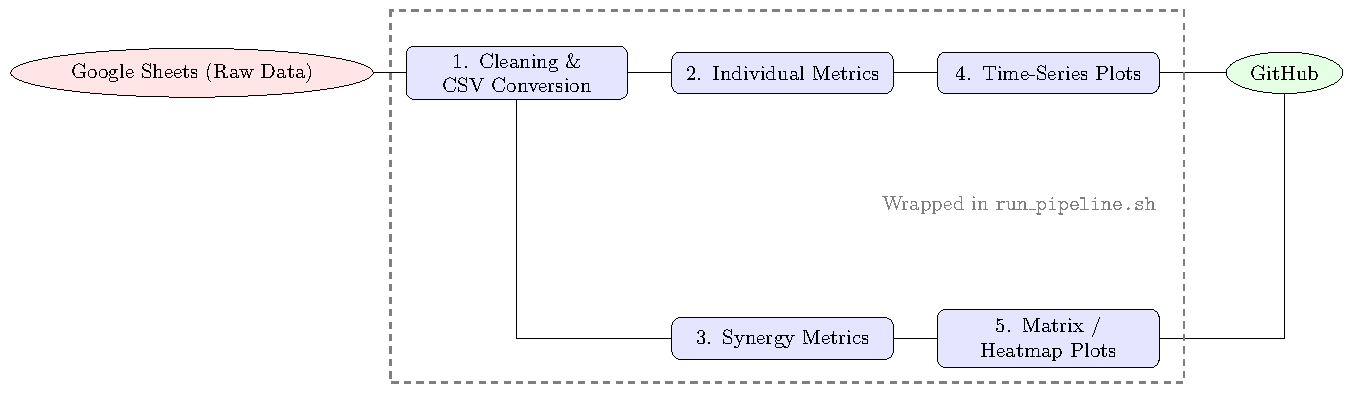
\includegraphics[width=0.9\textwidth]{flowchart.pdf}
    \end{center}
    
    \begin{columns}[t]
    \begin{column}{0.5\textwidth}
    \textbf{Aim of pipeline}
    \begin{itemize}
    		\item Ensure a consistent, reproducible and automatic execution environment.
    		\item Compute individual metrics of each player (ELO, goals scored by position, games played by position, etc.).
    		\item Compute metrics describing team performance (team wins, team clutch wins, goals conceded by team, etc.).
    		\item Plot the evolution of each metric during the season.
    \end{itemize}
    \end{column}
    
    \begin{column}{0.5\textwidth}
    \textbf{Workflow automation}
    \begin{itemize}
    		\item Pipeline is structured in modular Python codes, each one computing or plotting different metrics.
    		\item \texttt{.nc} files from \texttt{xarray} package are used to store and load data.
        \item \texttt{.sh} scripts execute the chain sequentially.
        \item Git hooks automatically push new plots to the website.
    \end{itemize}
    \end{column}
    \end{columns}

\end{frame}

% Slide 8: Automation \& GitHub
\begin{frame}[fragile]{Pipeline Orchestration \& Execution}
	\begin{block}{Running the pipeline}
        The pipeline is triggered directly from the terminal. The script sequentially executes the modular Python components:
        \begin{semiverbatim}
        \textcolor{green}{\$} ./pipeline.sh [-s]
        \end{semiverbatim}
	The optional command allows to specify the season number to compute. If no flag is specified, the analysis is conducted with the data available for all seasons, returning the historical trends.
    \end{block}
    \begin{block}{Uploading to \texttt{git}}
    An additional file runs the commands to include all generated files in \texttt{git}, which is then used to update the \href{https://www.github.com/pgrebolt/ICEChampionsLeague}{GitHub repository}.
        \begin{semiverbatim}
        \textcolor{green}{\$} ./add_to_git.sh
        \end{semiverbatim}
    \end{block}
\end{frame}


% --- SLIDE 2: XARRAY & DATA STRUCTURE ---
\begin{frame}{Data Storage: Why Xarray?}

\fontsize{7pt}{9pt}\selectfont

    \begin{columns}[T]
        \begin{column}{0.6\textwidth}
            \textbf{xarray} (NetCDF) is used for high-dimensional data handling. One code can generate \texttt{.nc} files that can be read by other codes to proceed with the analysis. \texttt{xarray} objects allow for easy slicing: \texttt{data.sel(player='Alice')}. Two kinds of \texttt{xarray} objects are used depending on individual/synergy metrics. Storage of \texttt{.nc} allow an easy access to player stats if new analysis codes are created.
            
            \vspace{1em}
            \textbf{Structure 1: Individual Performance}
            \begin{itemize}
                \item \textbf{Dimensions:} $(\text{Player}, \text{Match number})$
                \item \textbf{Variables} (per position and in any position)\textbf{:} games played, number of wins, win ratio, total goals scored, goals scored per game, goals received, goals received per game, $ELO_\text{Atk}$, $ELO_\text{Def}$, $ELO_\text{Weighted}$
            \end{itemize}

            \textbf{Structure 2: Synergy Matrix}
            \begin{itemize}
                \item \textbf{Dimensions:} $(\text{Player}_i, \text{Player}_j)$
                \item \textbf{Variables:} games played together, win rate, number of close matches, win rate in close matches, received goals, number of goals scored to a defender rival, number of clean sheets, team rate of clean sheets
            \end{itemize}
		\end{column}
     
        \begin{column}{0.4\textwidth}
            \centering
            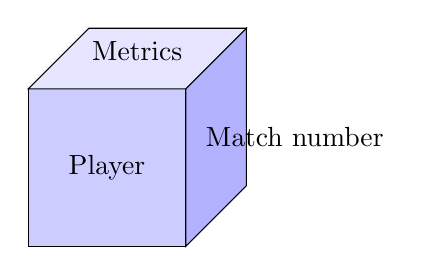
\begin{tikzpicture}
                % Simple 3D Cube to represent Data Tensor
                \draw[fill=blue!20] (0,0,0) -- (2,0,0) -- (2,2,0) -- (0,2,0) -- cycle;
                \draw[fill=blue!30] (2,0,0) -- (2,0,-2) -- (2,2,-2) -- (2,2,0) -- cycle;
                \draw[fill=blue!10] (0,2,0) -- (2,2,0) -- (2,2,-2) -- (0,2,-2) -- cycle;
                \node at (1,1,0) {Player};
                \node at (3, 1,-1) {Match number};
                \node at (1,2.1,-1) {Metrics};
            \end{tikzpicture}
            \\ \vspace{0.5em}
            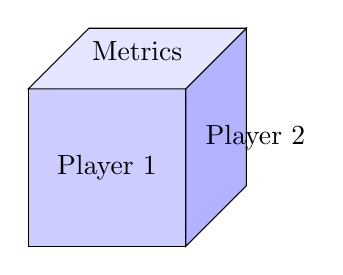
\begin{tikzpicture}
                % Simple 3D Cube to represent Data Tensor
                \draw[fill=blue!20] (0,0,0) -- (2,0,0) -- (2,2,0) -- (0,2,0) -- cycle;
                \draw[fill=blue!30] (2,0,0) -- (2,0,-2) -- (2,2,-2) -- (2,2,0) -- cycle;
                \draw[fill=blue!10] (0,2,0) -- (2,2,0) -- (2,2,-2) -- (0,2,-2) -- cycle;
                \node at (1,1,0) {Player 1};
                \node at (2.5,1,-1) {Player 2};
                \node at (1,2.1,-1) {Metrics};
            \end{tikzpicture}
        \end{column}
    \end{columns}

\textit{Note:} a \textit{close match} is a match with the result being 3-2 or 2-3. Alternatively, a \textit{clean sheet} is a won match with the result being 3-0 or 0-3.

\end{frame}

% ============================================================================
% SECTION 3: STATISTICAL ANALYSIS OF >1000 MATCHES
% This is the core "Results" section.
% ============================================================================
\section{Data Analysis \& Historical Trends}

% Slide 5: The ELO Distribution
\begin{frame}{Historical ELO distribution}
\centering
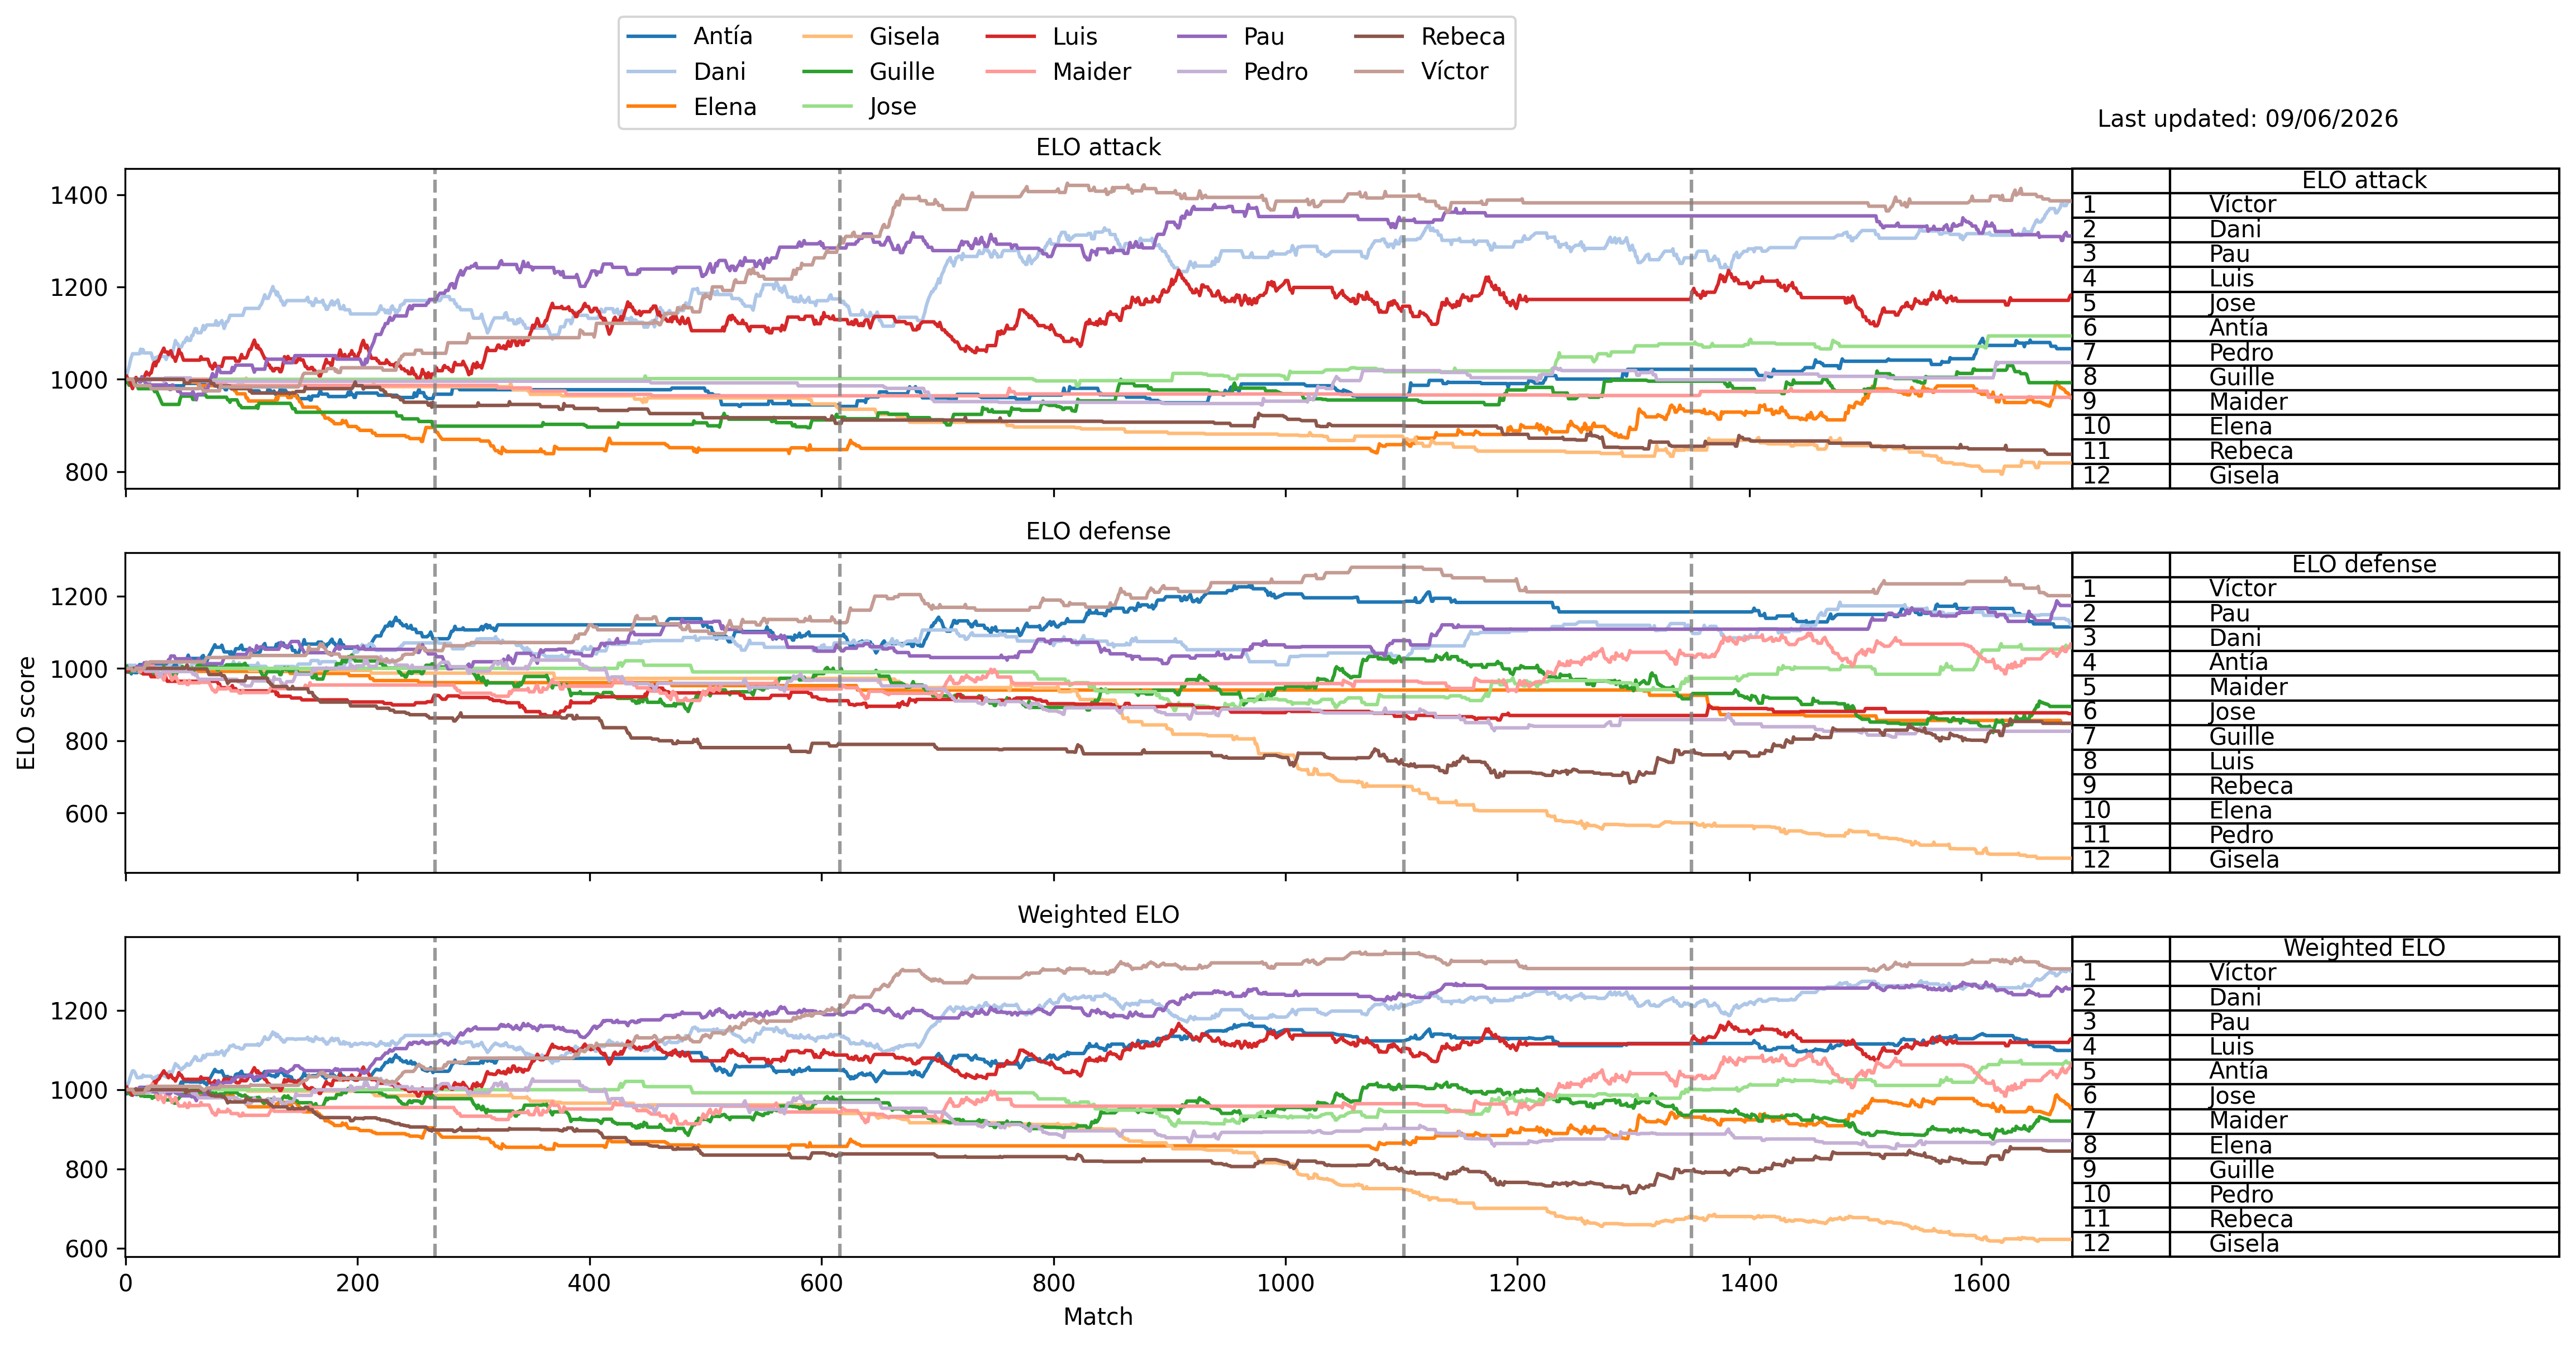
\includegraphics[width = \textwidth]{../results/historical/ELO_stats_historical.png}
\tiny{\textit{Note:} only players who played at least 20\% of the maximum number of games played are shown in plots.}
\end{frame}


\begin{frame}{Beyond ELO: Deconstructing Player Profiles}

    While the ELO rating provides a macroscopic measure of overall skill, other metrics can be defined to isolate specific strengths, weaknesses, and playstyles.

    \vspace{0.5em}
    \begin{columns}[T]
        % --- Left Column: General Metrics ---
        \begin{column}{0.48\textwidth}
            \begin{block}{Global Observables}
                Metrics calculated independent of position:
                \vspace{0.5em}
                \begin{itemize}
                    \item \textbf{Win Rate:} \\
                    $\frac{\text{Games Won}}{\text{Total Games}}$
                    \vspace{0.5em}
                    \item \textbf{Scoring Rate:} \\
                    $\frac{\text{Total Goals Scored}}{\text{Total Games}}$
                \end{itemize}
            \end{block}
        \end{column}

        % --- Right Column: Positional Metrics ---
        \begin{column}{0.5\textwidth}
            \begin{block}{Positional Specificity}
                Metrics isolated by role $i \in \{\text{Atk}, \text{Def}\}$:
                \vspace{0.5em}
                \begin{itemize}
                    \item \textbf{Offensive power:} \\
                    $\frac{\text{Goals Scored as } i}{\text{Games Played as } i}$
                    \vspace{0.5em}
                    \item \textbf{Defensive power:} \\
                    $\frac{\text{Goals Conceded as } i}{\text{Games Played as } i}$
                \end{itemize}
            \end{block}
        \end{column}
    \end{columns}

    \vspace{1em}
    \textit{Note:} By cross-referencing these normalized rates, players can be classified in archetypes (e.g., the "Highly Offensive Defender").

\end{frame}

\begin{frame}{Historical stats distribution}
\centering
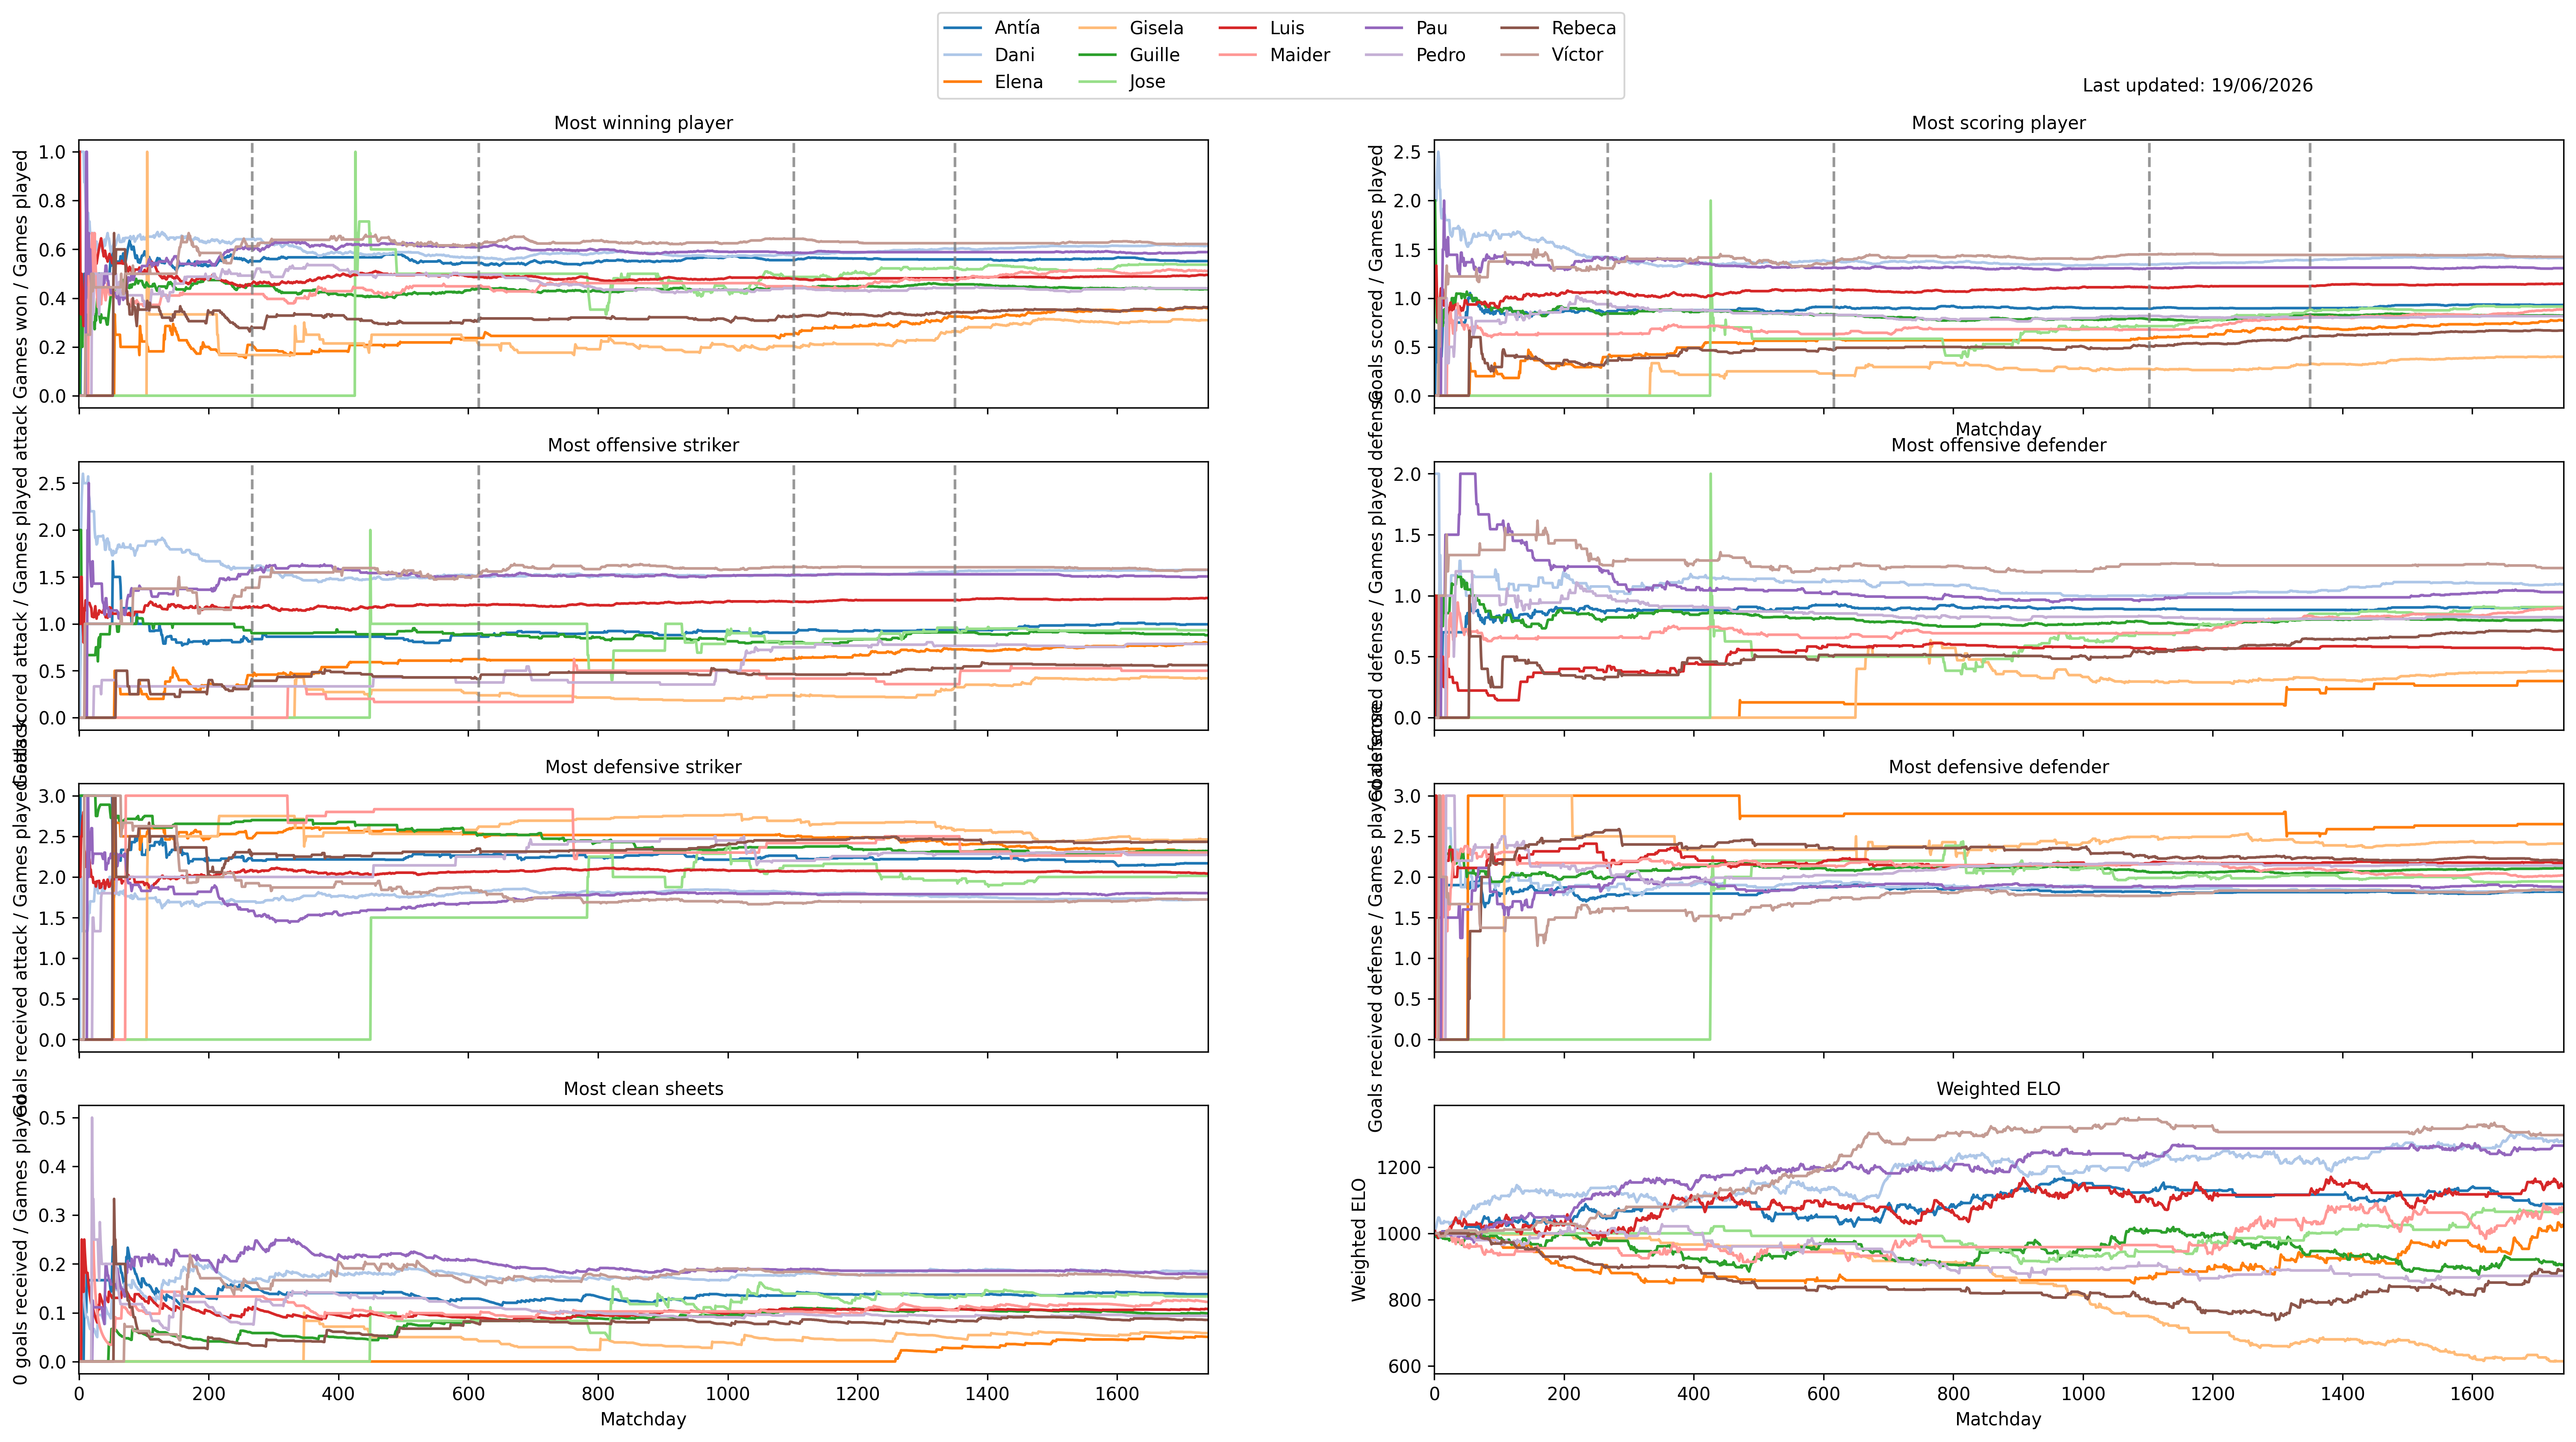
\includegraphics[width = \textwidth]{../results/historical/winplayed_stats_historical.png}
\end{frame}

% Slide 7: Synergy & Team Dynamics
\begin{frame}{Team dynamics}

\fontsize{7pt}{9pt}\selectfont

\begin{columns}[t]
\begin{column}{0.33\textwidth}
\centering
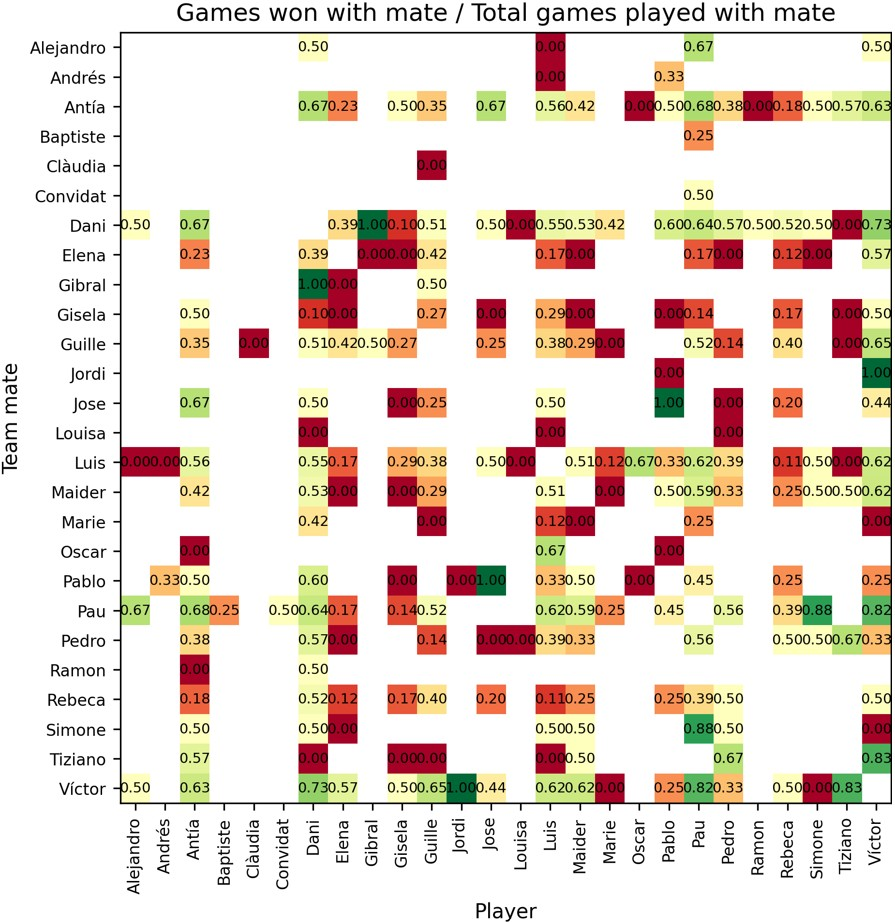
\includegraphics[width = \textwidth]{team_winning_ratio.jpeg}
Ratio of games won by each team, regardless of the position of players. This shows primary synergies between players.
\end{column}

\begin{column}{0.33\textwidth}
\centering
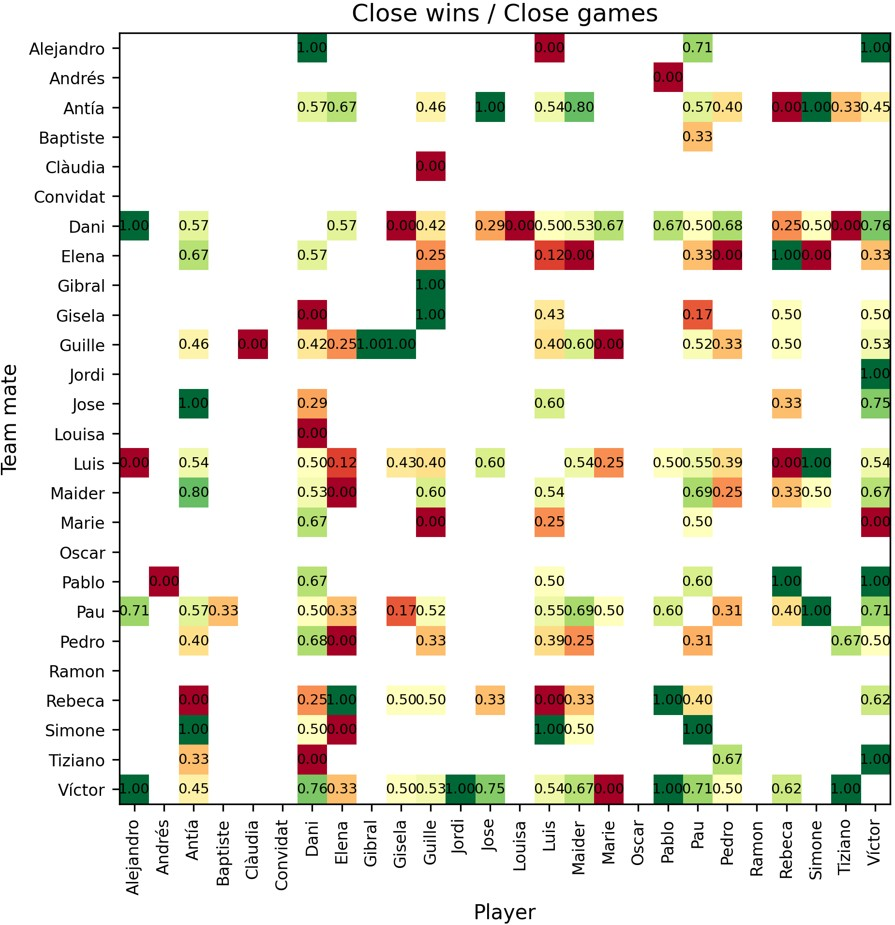
\includegraphics[width = \textwidth]{team_closewins_ratio.jpeg}
Ratio of close games won by each team, regardless of the position of players. A close game is that with result 3-2 or 2-3. This sketches which teams handle best winning under pressure.
\end{column}

\begin{column}{0.33\textwidth}
\centering
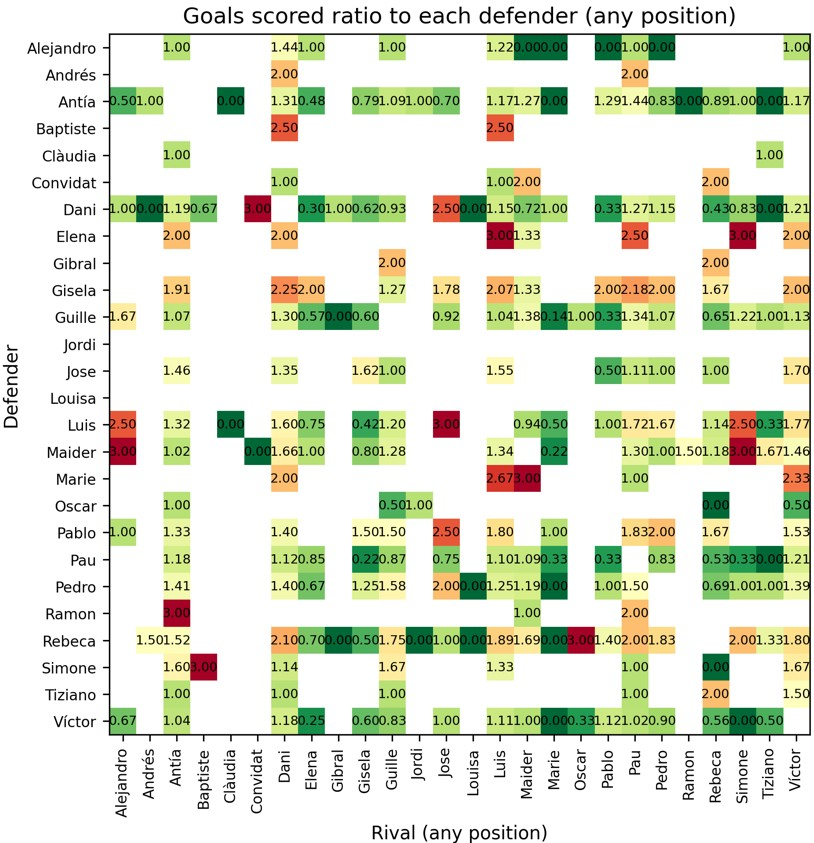
\includegraphics[width = \textwidth]{goals_conceded_defender_ratio.jpeg}
Number of goals conceded by each defender, for each rival. This allows to see which player is more prone to score goals to a given defender.
\end{column}

\end{columns}
\end{frame}

% ============================================================================
% SECTION 4: MACHINE LEARNING MODEL
% This is the core "Results" section.
% ============================================================================
\section{Machine Learning modelization}

% --- SLIDE 1: PROBLEM FORMULATION & FEATURES ---
\begin{frame}{Formulating the ML Problem}
\fontsize{8pt}{9pt}\selectfont

    \noindent\textbf{Goal:} Predict the Win/Loss outcome for Team A prior to the match starting.
    
    \noindent\textbf{Method:} Used XGBoost classifier. Python code based on \href{https://github.com/NunonuN/ml-playground}{\texttt{ml-playground}} GitHub repo.

    \noindent\textbf{The Feature Vector ($\vec{X}$):} 
    The models are trained with a set of parameters describing the individual and collective capabilities of players. The first $30\%$ games are removed to allow for parameters stabilization. The remaining set is split in 90:10 train:test split. Parameters used:

%considered_stats_teams = ['ELOAttackDefenseDifference','ELODefenseAttackDifference','ELODifference','WeightedELODifference',                          'WinsDifference', 'CloseWinsDifference', 'NeatGoalsAttackDifference', 'NeatGoalsDefenseDifference','WinsMatchdayDifference',                          'ReceivedGoalsDefenseDefenseDifference', 'ReceivedGoalsAttackDefenseDifference']
\begin{columns}[T]
        % --- Left Column ---
        \begin{column}{0.5\textwidth}
            \begin{block}{Skill Gradients ($\Delta$ELO)}
                \begin{itemize}
                    \item Overall $\Delta$ELO
                    \item Weighted $\Delta$ELO
                    \item Attacker (A) vs. Defender (B) $\Delta$ELO
                    \item Defender (A) vs. Attacker (B) $\Delta$ELO
                \end{itemize}
            \end{block}
            
            \begin{block}{Historical Momentum ($\Delta$Wins)}
                \begin{itemize}
                    \item Total Wins Difference
                    \item Close Wins (Clutch) Difference
                    \item Matchday Form (Wins) Difference
                \end{itemize}
            \end{block}
        \end{column}
        
        % --- Right Column ---
        \begin{column}{0.5\textwidth}
            \begin{block}{Scoring/Defensive Metrics ($\Delta$Goals)}
                \begin{itemize}
                    \item Attacker "Neat Goals" Difference
                    \item Defender "Neat Goals" Difference
                    \item Clean Sheets Difference
                    \item Def. vs Def. Goals Conceded Diff.
                    \item Atk. vs Def. Goals Conceded Diff.
                \end{itemize}
            \end{block}
		    \vspace{1em}
		    \textit{\small Note: All features represent the differencial {Team A--Team B}. They are standardized ($\mu=0, \sigma=1$) to ensure scale invariance across the classifiers.}
        \end{column}
    \end{columns}

\end{frame}

% ============================================================================
% SLIDE 1: XGBOOST PERFORMANCE DIAGNOSTICS
% ============================================================================
\begin{frame}{XGBoost Performance Diagnostics}

\fontsize{7pt}{8pt}\selectfont


    The \textbf{XGBoost classifier} achieves a highly optimized balance between sensitivity and specificity, which is crucial for handling the inherent statistical variance in sports data.

    \begin{columns}
        % --- Left Column: Metrics & Interpretation ---
        \begin{column}{0.3\textwidth}
            \begin{block}{Model Evaluation Metrics}
                \tiny
                Evaluated via 5-Fold Cross-Validation:
				\tiny{
				\centering
                \begin{tabular}{cccc}
                \hline 
                 & Precision & Recall & F1-score \\ 
                \hline 
                Loss & 0.68 & 0.76 & 0.72 \\ 
                Win & 0.6 & 0.5 & 0.54 \\ 
                \end{tabular} 
                }
            \end{block}
            \vspace{0.5em}
            \begin{itemize}
            \item Training size: 675. Test size: 120
            \item \footnotesize Accuracy: proportion of correct classifications
            \item \footnotesize Recall: proportion of actual positives correctly classified as positives
            \item \footnotesize F1-score: balanced model performance metric
            \item \footnotesize \textbf{ROC Curve:} AUC$\sim 0.72$. Notable class separability under asymmetric baseline conditions.
            \end{itemize}
        \end{column}
        
        % --- Right Column: Visual Diagnostics (Stacked Plots) ---
        \begin{column}{0.35\textwidth}
            \centering
            % Top Plot: Confusion Matrix
            \includegraphics[width=\textwidth, keepaspectratio]{../results/ML/Confusion_Matrix_test_winning.png} \\
         \end{column}
         \begin{column}{0.25\textwidth}
            % Bottom Plot: ROC Curve
            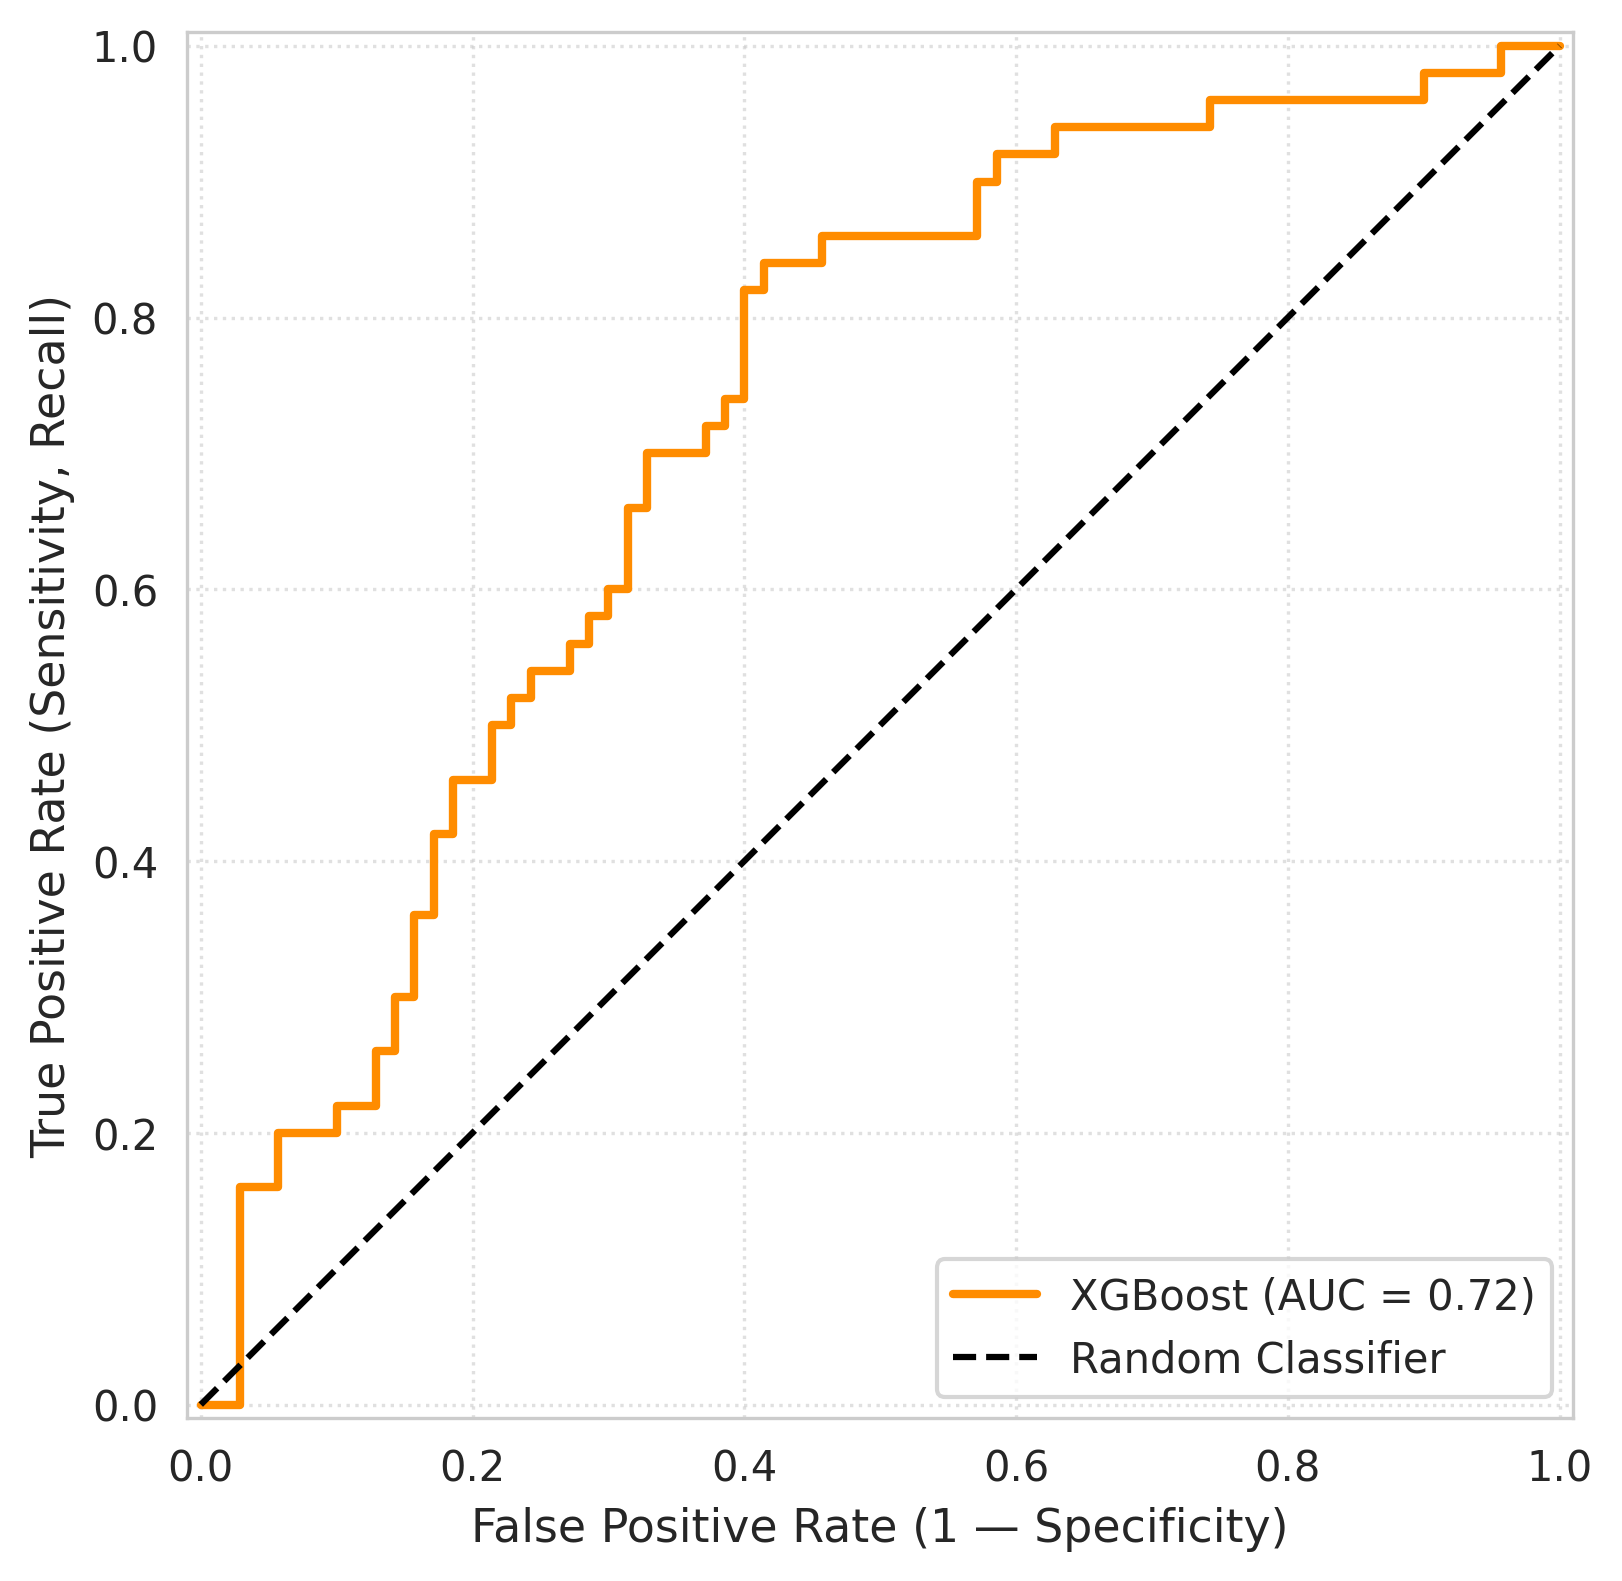
\includegraphics[width=\textwidth, keepaspectratio]{../results/ML/ROC_AUC_winning.png}
        \end{column}
    \end{columns}
\end{frame}

% ============================================================================
% SLIDE 2: SHAP FEATURE ATTRIBUTION
% ============================================================================
\begin{frame}{Physical Interpretation: SHAP Feature Attribution}

\fontsize{7pt}{8pt}\selectfont

    \textit{How does the algorithm weigh individual gradients to calculate a prediction?}
    
    \vspace{0.5em}
	 \textbf{SHAP (Shapley Additive Explanations)} was implemented to map the exact margin of contribution for each differential variable.

    \vspace{0.5em}
    \begin{columns}[T]
        % --- Left Column: SHAP Beeswarm Plot Summary ---
        \begin{column}{0.5\textwidth}
            \centering
            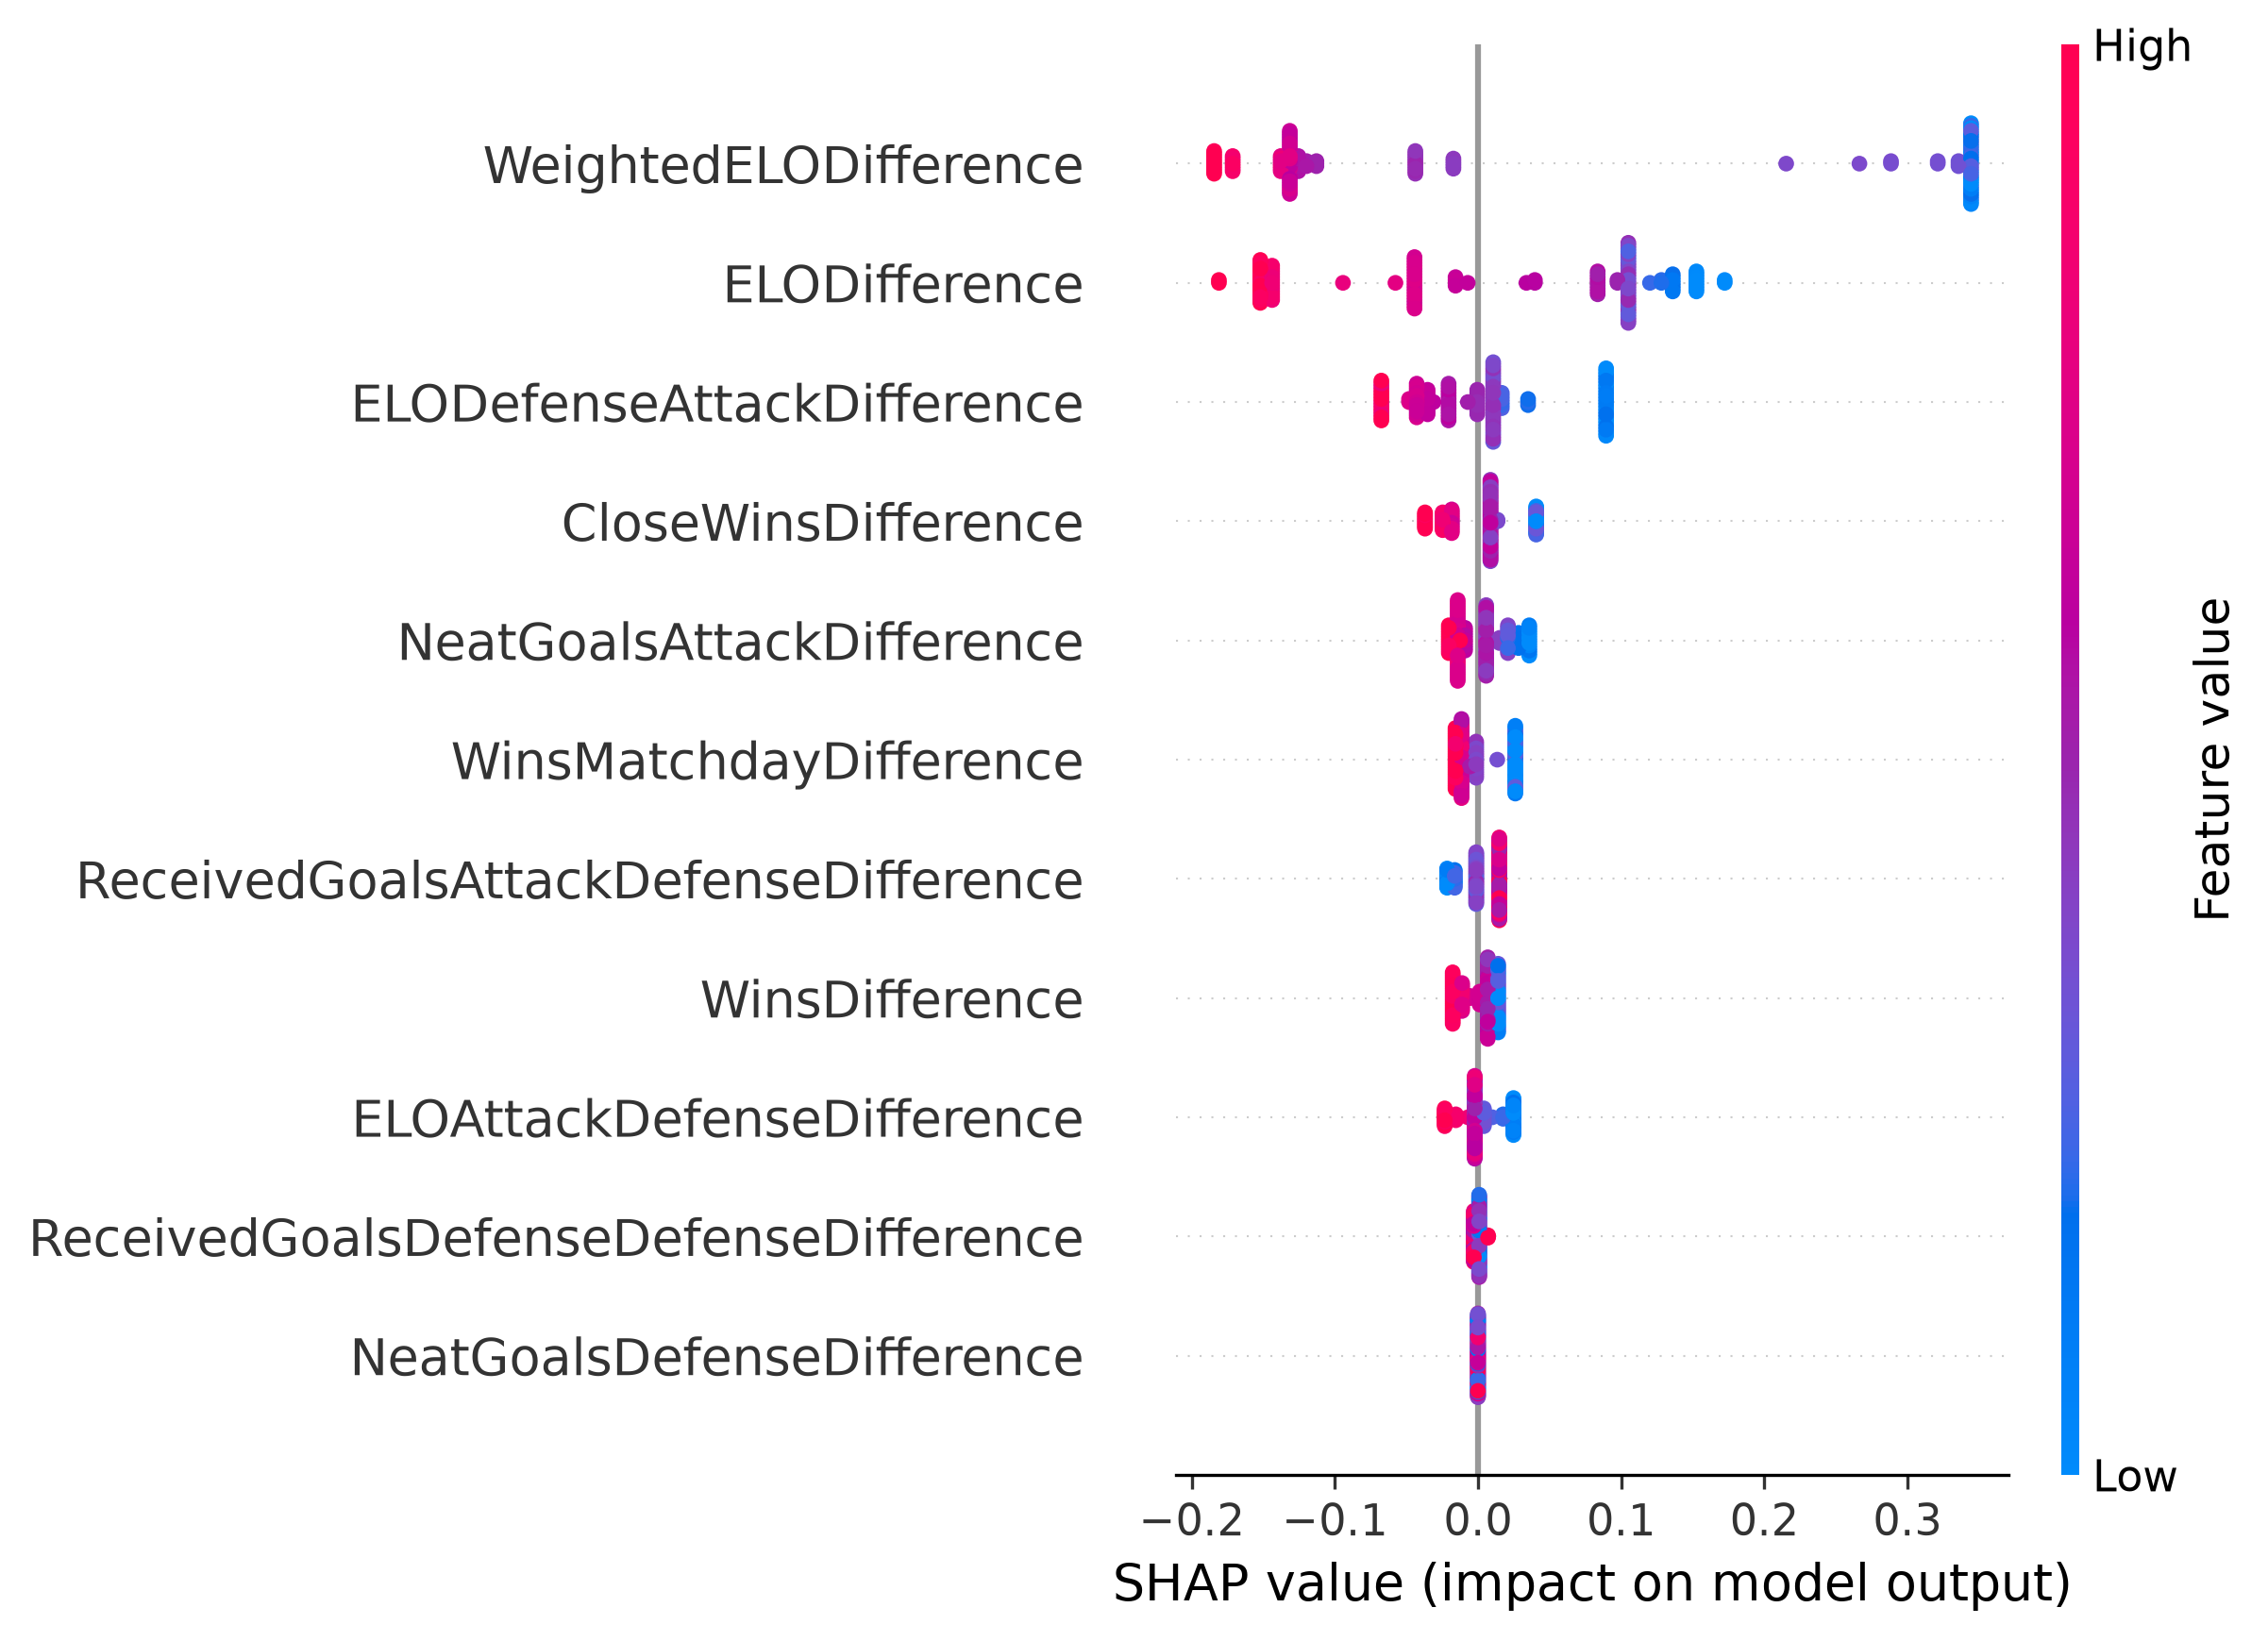
\includegraphics[width=\textwidth, keepaspectratio]{../results/ML/shap_summary_winning.png} \\
        \end{column}
        
        % --- Right Column: Physical Insights ---
        \begin{column}{0.5\textwidth}
            \begin{block}{Key Physical Takeaways}
                \footnotesize
                \begin{itemize}
                    \item \textbf{Dominant Macro-State:} 
                    \texttt{WeigthedELODifference} drives the global baseline attribution, acting as the primary system gradient. Overall experience is important.
                    
                    \item \textbf{The Synergy Factor:} 
                    Total ELO team difference (\texttt{ELODifference}) is the second most important factor, deciding narrow-margin matches between closely ranked opponents.
                    
                    \item \textbf{Defensive Lock:} 
                    Direct difference between defender and attacker (\texttt{ELODefenseAttackDifference}) also play a relevant role in match outcome prediction.
                \end{itemize}
            \end{block}
            
        \end{column}
    \end{columns}
\end{frame}

% ============================================================================
% SECTION 5: CONCLUSION
% ============================================================================
\section{Conclusion}
\begin{frame}{Conclusions \& Core Takeaways}

%\fontsize{7pt}{9pt}\selectfont

    \vspace{0.8em}
    \begin{columns}[T]
        % --- Left Column: Methodology & Logic ---
        \begin{column}{0.48\textwidth}
            \begin{block}{Methodological Contributions}
                \small
                \begin{itemize}
                    \item \textbf{State Decoupling:} Successfully isolated micro-level individual contributions ($r_i$) from macro-level team outcomes ($W$).
                    \item \textbf{Conservation \& Balance:} Introduced the ELO scoring to classify player positional level, overcoming uneven number of games played.
                \end{itemize}
            \end{block}
        \end{column}
        
        % --- Right Column: Code & Pipeline ---
        \begin{column}{0.48\textwidth}
            \begin{block}{Software \& Pipeline Architecture}
                \small
                \begin{itemize}
                    \item \textbf{Atomic Execution:} Created a unified shell interface (\texttt{pipeline.sh}) that guarantees exact reproducibility across modular scripts.
                    \item \textbf{Predictive Mapping:} Proven that tree-boosting (XGBoost) operating on feature differentials ($\Delta \vec{X}$) can forecast foosball game results.
                \end{itemize}
            \end{block}
        \end{column}
    \end{columns}

    \vspace{1em}
    \begin{alertblock}{Takeaways}
	This project has fully exploited the few recorded data from each game (goals scored by each player) to build a full competition report. The design has always focused so that data could be easily recorded and the new ELO updates could be accessed soon after the matchday was completed, which is assured by the modular pipeline.
    \end{alertblock}

\end{frame}

\end{document}